
\documentclass{beamer}
\usepackage[utf8]{inputenc}

\usetheme{Madrid}
\usecolortheme{default}
\usepackage{amsmath,amssymb,amsfonts,amsthm}
\usepackage{mathtools}
\usepackage{txfonts}
\usepackage{tkz-euclide}
\usepackage{listings}
\usepackage{adjustbox}
\usepackage{array}
\usepackage{tabularx}
\usepackage{gvv}
\usepackage{lmodern}
\usepackage{circuitikz}
\usepackage{tikz}
\usepackage{graphicx}
\setbeamertemplate{page number in head/foot}[totalframenumber]
\usepackage[T1]{fontenc}
\usepackage{tcolorbox}
\tcbuselibrary{minted,breakable,xparse,skins}

\definecolor{bg}{gray}{0.95}
\DeclareTCBListing{mintedbox}{O{}m!O{}}{%
  breakable=true,
  listing engine=minted,
  listing only,
  minted language=#2,
  minted style=default,
  minted options={%
    linenos,
    gobble=0,
    breaklines=true,
    breakafter=,,
    fontsize=\small,
    numbersep=8pt,
    #1},
  boxsep=0pt,
  left skip=0pt,
  right skip=0pt,
  left=25pt,
  right=0pt,
  top=3pt,
  bottom=3pt,
  arc=5pt,
  leftrule=0pt,
  rightrule=0pt,
  bottomrule=2pt,
  toprule=2pt,
  colback=bg,
  colframe=orange!70,
  enhanced,
  overlay={%
    \begin{tcbclipinterior}
    \fill[orange!20!white] (frame.south west) rectangle ([xshift=20pt]frame.north west);
    \end{tcbclipinterior}},
  #3,
}

% Code style
\lstset{
    language=C,
    basicstyle=\ttfamily\small,
    keywordstyle=\color{blue},
    stringstyle=\color{orange},
    commentstyle=\color{green!60!black},
    numbers=left,
    numberstyle=\tiny\color{gray},
    breaklines=true,
    showstringspaces=false,
}

% Title info
\title %optional
{Discrete - 1.2.18}
\date{March 26, 2026}
\author % (optional)
{EE25BTECH11018 - Darisy Sreetej}

\begin{document}

\frame{\titlepage}

\begin{frame}{Question}
The z-transform \textbf{X[z]} of a sequence x[n] is given by \textbf{X[z]} = $\frac{0.5}{1 - 2 z ^{-1}}$
. It is given that the region of convergence of \textbf{X[z]} includes the unit circle. The value of x[0] is:
 \begin{enumerate}
\item   $- 0.5$ 
\item   $0$
 \item $0.25$
\item  $0.5$
 \end{enumerate}
 \hfill(EC 2007)
\end{frame}
\begin{frame}{Solution}
The Z-transform of a discrete-time sequence x[n] is defined as :
\begin{align}
    \mathbf{X(z)} = \sum_{n=-\infty}^{\infty} x[n]  z^{-n}
\end{align}
The ROC (region of covergence) is the set of values of z in the complex plane for which the Z-transform sum converges absolutely (i.e., gives a finite value)

\quad

A pole of a Z-transform is defined as the value of z that makes the X[z] to blow up to infinity (i.e., denominator of X[z] equal to zero) 
\end{frame}
\begin{frame}{Solution}
Set :
\begin{align*}
& 1 - 2z^{-1} = 0 \\ 
&\Rightarrow 2z^{-1} = 1\\
&\Rightarrow z^{-1} = \frac{1}{2} 
\end{align*}
\begin{align}
&\Rightarrow z = 2
\end{align}

Therefore ,  there is a single pole at z = 2, which lies at a radius of $|z|$ = 2 in the complex plane.

\end{frame}

\begin{frame}{Solution}
The pole of $X(z)$ is at $z = 2$, so two possible ROCs exist:

\begin{align}
    \text{ROC}_1 &: |z| > 2 \quad \text{(right-sided, causal)} \\
    \text{ROC}_2 &: |z| < 2 \quad \text{(left-sided, anti-causal)}
\end{align}

Since the unit circle $|z| = 1$ must lie inside the ROC, and:
\begin{align}
    |z| = 1 < 2
\end{align}

The unit circle lies inside $|z| < 2$, NOT inside $|z| > 2$.\\


    ROC : $|z| < 2$ 
\begin{align}
\text{This means } x[n] \text{ is a } \textbf{left-side(anti-causal)} \text{ sequence}.
\end{align}
\end{frame}

\begin{frame}{Solution}


Given Expression , 


\begin{align}
    \mathbf{X[z]} = \frac{0.5}{1 - 2 z ^{-1}} 
\end{align}

by multiplying numerator and denominator with z 
\begin{align}
    \mathbf{X[z]} = \frac{0.5z}{z-2} \\
    \mathbf{X[z]} = -0.5\brak{\frac{z}{2}}\brak{\frac{1}{1-\frac{z}{2}}}
\end{align}
\end{frame}

\begin{frame}{Solution}
Expanding $\brak{\frac{1}{1-\frac{z}{2}}}$ using Geometric Series
\begin{align}
\Rightarrow \frac{1}{1 - \frac{z}{2}} = \sum_{k=0}^{\infty} \brak{\frac{z}{2}}^k
\end{align}
(Since , $|z| < 2  \Rightarrow   |\frac{z}{2}| < 1 $ )

\begin{align}
\mathbf{X(z)} = -0.5  \frac{z}{2} \sum_{k=0}^{\infty} \brak{\frac{z}{2}}^k \\
= -0.5 \sum_{k=0}^{\infty} \frac{z^{k+1}}{2^{k+1}}
\end{align}

by the definition of Z-transform 
\begin{align}
X(z) = \sum_{n=-\infty}^{\infty} x[n] z^{-n}
\end{align}



\end{frame}

\begin{frame}{Solution}
On comparing powers
\begin{align}
z^{k+1} = z^{-n} \Rightarrow n = -(k+1)
\end{align}

\begin{align}
\text{Hence, } k = -n - 1 \\
x[n] = -0.5 \cdot 2^n, \quad \text{for } n \le -1
\end{align}

\begin{align}
\therefore \quad 
x[n] = -0.5 \cdot 2^n \, u[-n-1]
\end{align}
where $u[-n-1]$ is the unit step function defined as:
\begin{align}
u[-n-1] = \begin{cases} 
1 & n \leq -1 \\ 
0 & \text{otherwise} 
\end{cases}
\end{align}
\end{frame}

\begin{frame}{Solution}
    \begin{align}
x[0] &= -0.5\brak{2^{0}}\brak{ u[-0-1]}\\
&= -0.5\brak{1}\brak{ u[-1]}\\
&= -0.5\brak{1}\brak{0} = 0\\
\text{Therefore, } x[0] &= 0  \text{  (Option 2)}
\end{align}
\end{frame}


\begin{frame}[fragile]
    \frametitle{Python code}
    \begin{lstlisting}[language=Python]
import numpy as np
import matplotlib.pyplot as plt
from scipy import signal

# Given
num = [0.5]
den = [1, -2]

# Poles
_, poles, _ = signal.tf2zpk(num, den)

# Left-sided inverse Z-transform
n_vals = np.arange(-7, 3)
x_n = np.array([-0.5 * (2.0**n) if n <= -1 else 0.0 for n in n_vals])
print(f"x[0] = {x_n[n_vals == 0][0]}")
    \end{lstlisting}
\end{frame}

\begin{frame}[fragile]
    \frametitle{Python code}

    \begin{lstlisting}[language=Python]
#plotting
fig, axes = plt.subplots(1, 2, figsize=(12, 5))
fig.suptitle(r"Z-Transform: $X(z) = \frac{0.5}{1-2z^{-1}}$,  ROC: $|z|<2$ (Left-sided)",
fontsize=13, fontweight='bold')

ax1 = axes[0]
ax1.stem(n_vals, x_n, basefmt='k-', linefmt='steelblue', markerfmt='bo')
ax1.scatter([0], [0], color='red', s=120, label='x[0] = 0')
ax1.axvline(0, linestyle='--', linewidth=1)
ax1.set_title(r"x[n] vs n")
ax1.set_xlabel("n")
ax1.set_ylabel("x[n]")
ax1.legend()
ax1.grid(True)

    \end{lstlisting}
\end{frame}

\begin{frame}[fragile]
    \frametitle{Python code}

    \begin{lstlisting}[language=Python]
ax2 = axes[1]
theta = np.linspace(0, 2*np.pi, 300)
# ROC shading
roc_circle = plt.Circle((0, 0), abs(poles[0]), alpha=0.15,label='ROC: |z| < 2')
ax2.add_patch(roc_circle)

# Unit circle
ax2.plot(np.cos(theta), np.sin(theta), linestyle=':', linewidth=1.5,label='Unit Circle')

# Pole
ax2.scatter(np.real(poles), np.imag(poles), s=120,label='Pole at z=2')

# Add legend
ax2.legend()


\end{lstlisting}
\end{frame}
\begin{frame}[fragile]
    \frametitle{Python code}
    \begin{lstlisting}[language=Python]
ax2.axhline(0, linewidth=0.5)
ax2.axvline(0, linewidth=0.5)
ax2.set_title("Pole-Zero Plot")
ax2.set_xlabel("Real")
ax2.set_ylabel("Imaginary")
ax2.grid(True)
ax2.set_aspect('equal')
ax2.set_xlim(-3, 3)
ax2.set_ylim(-3, 3)

plt.tight_layout()
plt.show()
    \end{lstlisting}
\end{frame}

\begin{frame}{Plot}
    \begin{figure}
        \centering
        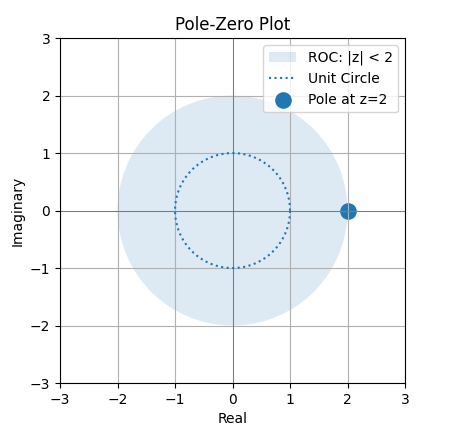
\includegraphics[width=0.726\linewidth]{plot1.png}
        \caption{Enter Caption}
        \label{fig:placeholder}
    \end{figure}
\end{frame}

\begin{frame}{Plot}
    \begin{figure}
        \centering
        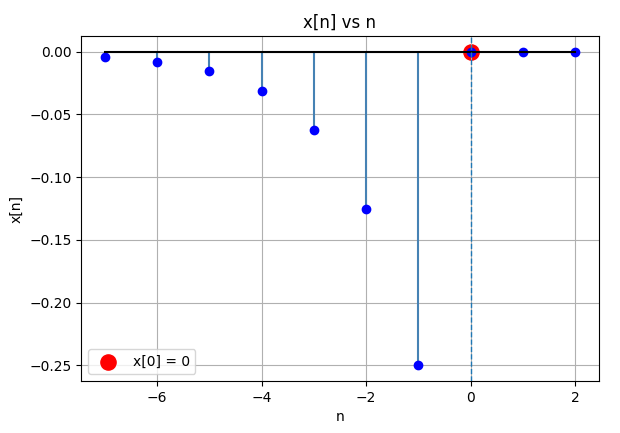
\includegraphics[width=0.90\linewidth]{plot2.png}
        \caption{Enter Caption}
        \label{fig:placeholder}
    \end{figure}
\end{frame}

\end{document}



